%\documentclass[draft,twoside,paper=a4,abstract=true,english,DIVcalc]{scrartcl}
\documentclass[twoside,paper=a4,abstract=true,english,DIV=calc]{scrartcl}
\usepackage[utf8]{inputenc}
\usepackage[T1]{fontenc}
\usepackage{babel}
\usepackage{graphicx}	
\usepackage{setspace}
	\doublespacing
\usepackage[colorinlistoftodos]{todonotes}
\usepackage[load-configurations=binary]{siunitx}
	\DeclareSIUnit\Molar{\textsc{m}}
\usepackage{microtype}
\usepackage{textcomp} % to suppress warnings from microtype
\usepackage{svn-multi}
\usepackage{subfig}
\usepackage{fancyhdr}
\usepackage{tikz}
\usepackage{pgfplots}
	\usepgfplotslibrary{groupplots}
\usepackage[numbers,square,sort&compress]{natbib}
\usepackage{scrtime}
\usepackage{lastpage}
\usepackage{xspace}
\usepackage[autostyle=true]{csquotes}
%\usepackage{endfloat}
\usepackage{hyperref}
 
% Subversion Information
\svnidlong
{$HeadURL$}
{$LastChangedDate$}
{$LastChangedRevision$}
{$LastChangedBy$}
\svnid{$Id$}
 
\pagestyle{fancy}
\fancyfoot{}
\fancyfoot[OR]{\tiny Typeset on \today\ at \thistime\ from \href{\svnkw{HeadURL}}{SVN-Version \svnkw{LastChangedRevision}} | Page \thepage\ of \pageref{LastPage}}
\fancyfoot[EL]{\tiny Page \thepage\ of \pageref{LastPage} | Typeset on \today\ at \thistime\ from \href{\svnkw{HeadURL}}{SVN-Version \svnkw{LastChangedRevision}}}
 
\newcommand{\imsize}{\linewidth}
\newlength\imagewidth		% needed for scalebars
\newlength\imagescale		% ditto

\newcommand{\footremember}[2]{\footnote{#2}\newcounter{#1}\setcounter{#1}{\value{footnote}}}
\newcommand{\footrecall}[1]{\footnotemark[\value{#1}]}

\newcommand{\superscript}[1]{\ensuremath{^{\textrm{#1}}}}
\newcommand{\subscript}[1]{\ensuremath{_{\textrm{#1}}}}

\newcommand{\ie}{i.\,e.\ }
\newcommand{\eg}{e.\,g.\ }

\newcommand{\subfigureautorefname}{\figureautorefname} % make \autoref work with \subfloat

\newcommand{\numberofacini}{43}
\newcommand{\volume}{0.0015546092234} % cm^3, (mean acinar volume)
\newcommand{\std}{0.000624982186542} % (Standard deviation of acinar volumes)
\newcommand{\difference}{3.13348837209} % X times bigger (acinar volumes STEPanizer/MeVisLab-volumes)
 
\title{Assessing the volume and surface of individual acini in large tomographic datasets of rat lungs}
\subtitle{Stereological characterization of individual rat lung acini extracted from large ultrahigh resolution tomographic datasets}

\author{%
	David Haberthür\footremember{ana}{Institute of Anatomy, University of Bern, Switzerland}%
	\and Sébastien Barré\footrecall{ana}%
	\and Stefan Tschanz\footrecall{ana}%
	\and Marco Stampanoni\footremember{psi}{Swiss Light Source, Paul Scherrer Institut, Villigen, Switzerland}\ \footremember{eth}{Institute for Biomedical Engineering, Swiss Federal Institute of Technology and University of Zürich, Switzerland}%
	\and Johannes C. Schittny\footrecall{ana}\ \footremember{contact}{Corresponding Author: Email: \href{mailto:schittny@ana.unibe.ch}{schittny@ana.unibe.ch}, Telephone: +41 31 631 46 35, Fax: +41 31 631 38 07, Address: Institute of Anatomy, University of Bern, Baltzerstrasse 2, CH-3012 Bern}%
	}

\begin{document}
\setcounter{secnumdepth}{-1} % No section numbering, please!
\renewcommand{\subsectionautorefname}{\sectionautorefname} % useful for \autoref
\renewcommand{\subsubsectionautorefname}{\sectionautorefname} % useful for \autoref
\maketitle
\begin{center}
\vfill
Typeset on \today\ at \thistime\ from Rev \svnkw{LastChangedRevision} (\svnday.\svnmonth.\svnyear\ \svnhour:\svnminute)
\vfill
To be submitted to the \emph{\href{http://jap.physiology.org/}{Journal of Applied Physiology}}, \emph{Innovative Techniques}
\vfill
\end{center}
\clearpage

\begin{abstract}
The pulmonary acinus represents the respiratory functional unit of the lung. Due to a restricted availability of high resolution imaging methods the knowledge about several biological parameters of  of the acini is limited. Single acini cannot be well characterized from two-dimensional physical sections, due to restrictions imposed by the sectioning method. Our new method builds upon high resolution three dimensional tomographic data obtained by synchrotron radiation based tomographic microscopy. We developed a method to isolate and analyze single acini, to assess their volume and surface and estimate the number of alveoli contained in them. In three-dimensional tomographic datasets we closed the transition between conducting and gas-exchanging airways bronchioles semi-automatically with three-dimensional discs acting as segmentation breakpoints. Our method makes it possible to extract individual acini for volume analysis, something which is not possible on two-dimensional data from single sections of the tissue. The automatic volume analysis of single acini was manually confirmed with stereological assessment. Our proposed method of analyzing single ventilatory units of the mammalian lung is by magnitudes faster than manual stereological analysis of tissue slices and allows to extract biological parameters which can not be extracted from classic single sections. Additionally, the method makes it possible to assess the development of the acini and structural changes in the functional lung units over the postnatal lung development.\todo{One paragraph, no more than 250 words, currently these are 218 words.}
\end{abstract}
	
\section{Keywords}
\begin{itemize}
	\item lung development,
	\item stereology
	\item tomography
	\item acinus
	\item visualization\todo{Three to five words that do not appear in the title or running head}
\end{itemize}
\clearpage
\listoftodos
\clearpage
\tableofcontents

\clearpage
\section{Introduction}
Due a restricted availability of high resolution three-dimensional imaging methods the knowledge about the development of the ventilatory functional unit of the lung is limited. These functional units of the lung parenchyma are the so-called pulmonary acini, which correspond to the gas-exchange volume in the lung which is ventilated by one purely conducting airway~\cite{Rodriguez1987}.

In the present manuscript we describe a method to isolate and analyze single acini from large high-resolution tomographic datasets. Using datasets obtained with synchrotron radiation based tomographic microscopy with enhanced field of view~\cite{Haberthuer2010a}, we extracted individual acini from rat lung samples throughout postnatal lung development. 

Extracting large amounts of single acini from physical sections of lung tissue is extremely time-consuming. \citet{Woodward2005} achieved three-dimensional reconstructions of three adult duck lungs using manual effort to trace serial sections of the tissue. Observing and tracing single acini on microscopy slides for the extraction of their volume is nearly impossible. \citet{Rodriguez1987} mention that they attempted a serial section-reconstruction of individual airways but resorted to a method with casting the airways system with silicon to assess the acini in rat and rabbits. In their publication they analyzed one animal for each species with very tedious manual labor, while unfortunately neither mentioning the exact rat strain nor the age of the animal\todo{Are there other publications giving numbers?}.

We propose a method to nondestructively characterize single acini with minimal manual work based on tomographic datasets. Since tomographic imaging of the lung tissue preserves the three-dimensional structure, single slices from the images can be extracted trivially easy and be used for precise analysis of the morphometry of structures in the lung tissue.

Since such virtual slices from tomographic datasets do not destroy the three-dimensional structure, we can thus isolate and analyze single acini with classic and accepted methods in both two and three dimensions. In addition to three-dimensional volume analysis through segmentation and voxel counting in a visualization software we performed standard stereological analysis~\cite{Hsia2010} to compare our results with an accepted ground truth. As stated by \citet{Hsia2010}, \blockquote{Stereology refers to the mathematical methods for analyzing properties of an irregular three-dimensional structure using two-dimensional planar sections obtained by physical or optical imaging techniques}.

Extracting single acini from the tomographic datasets enables us to perform such a stereological analysis to obtain a complete description of the ventilatory functional lung units including alveolar number\todo{Do we show alveolar numbers?}, surface and volume and compare how these values change during the postnatal lung development. Such a complete description is only possible with tomographic data, since the three-dimensional information in the sample is not destroyed, while otherwise---with classic microscopy-based analysis techniques---the lung tissue has to be sectioned, essentially destroying the tissue in the process. The manuscript at hand describes a stereological analysis of the volume of single functional units of the mammalian lung.

\subsection{Lung structure and the acini}
The airway structure of the mammalian lung is formed from dichotomous branches \cite{Weibel1991}, starting from the trachea. The first branching generations lead into the bronchi. With increasing depth into the airway tree, the airway diameter of the airways is reduced, the bronchi are divided into bronchioles, leading to the terminal bronchioles which then mark the end of the pipe-like purely conducting airways. The respiratory bronchioles mark the start of the gas-exchange region in the lung.

The change between purely conducting and gas-exchanging airways is marked by changes in the airway wall structure---alveolar outpouchings---and in the airway epithelium (see \autoref{fig:ManholeCoverExplanation}). After this point, the so-called acinar airways and all the airspace behind one of these points forms one functional lung unit, the so-called acinus. Observation of such changes in the airway wall make it possible to extract single acini from the three-dimensional tomographic datasets, as described later in Materials and Methods, \autoref{sec:materials and methods}.

The lung structure can be assessed using Stereology, as shown by \citet{Hsia2010} and \citet{Tschanz2002}. Such an analysis is generally based on two-dimensional physical sections of the sample, thus the extracted information is a two-dimensional description \blockquote[\cite{Tschanz2002}]{of the parenchymal air space geometry and, due to geometric laws, it is not allowed to extrapolate these two-dimensional statements directly to three-dimensional structures}. With stereological methods it is possible to extract global volume information, but it not easily feasible to extract such information from a functional subunit of an organ like the acini in the lung, since it cannot easily be assessed which detail on one microscopy slide belongs to which functional unit in the three-dimensional compound. With a three-dimensional segmentation we can extract virtual two-dimensional slices of single isolated functional units, thus for a first time enabling a precise stereological characterization of individual acini in the mammalian lung.

\section{Materials and Methods}
\label{sec:materials and methods}
\subsection{Rat lung samples}
The results shown in this manuscript have been obtained from lungs from three adult Sprague-Dawley rats at day 60 after birth. Animals were deeply anesthetized with a mixture of %
\SI{0.5}{\milli\gram\per\milli\litre} Acetylpromazine, %
\SI{5}{\milli\gram\per\milli\litre} Xylazine and %
\SI{50}{\milli\gram\per\milli\litre} Ketamine in %
\SI{0.9}{\percent} NaCl at \SIrange{1.5}{2.5}{\micro\litre} per \si{\gram} body weight. The lungs of the animals were instilled with \SI{2.5}{\percent} Glutaraldehyde in \SI{0.03}{\Molar} potassium-phosphate buffer (pH 7.4) at a constant pressure of \SI{20}{\centi\meter} water column. At this applied pressure, the rat lung reaches its mid-respiratory volume~\cite{Schittny1998}. The instillation was performed via tracheotomy after opening the chest cavity and setting a pneumothorax through perforation of the diaphragm. After instillation the lung was removed from the chest cavity and the instillation pressure was maintained during fixation (in the same fixative at \SI{4}{\celsius} for at least \SI{24}{\hour}) in order to prevent a recoiling of the lung~\cite{Tschanz2002}.

After fixation, the samples were prepared for tomographic imaging by post-fixation with \SI{1}{\percent} osmium acetate and staining with \SI{4}{\percent} uranyl nitrate to increase the x-ray absorption contrast. Using Histoclear (Merck KGaA, Darmstadt, Germany) as an intermedium the samples were then dehydrated in a graded series of ethanol and embedded in paraffin prior to mounting them onto standard scanning electron microscopy sample holders (PLANO GmbH, Wetzlar, Germany) with paraffin~\cite{Tsuda2008}.

The handling of animals before and during the experiments, as well as the experiments themselves, were approved and supervised by the Swiss Agency for the Environment, Forests and Landscape and the Veterinary Service of the Canton of Bern, Switzerland.

\subsection{Tomographic data acquisition}
The tomographic experiments were performed at the \href{http://www.psi.ch/sls/tomcat/}{TOMCAT beamline} at the \href{http://www.psi.ch/sls/}{Swiss Light Source}, \href{http://www.psi.ch/}{Paul Scherrer Institut}, Villigen, Switzerland~\cite{Stampanoni2006a}. The samples were scanned at an x-ray energy of \SI{20.0}{\kilo\electronvolt} corresponding to a wavelength of \(\lambda=\SI{0.62}{\angstrom}\). % \lambda = 1.24e-6 eV/m / 20 keV = 6.197796e-11 m = 0.6197796 Ångström

After penetration through the sample, the x-rays were converted into visible light by either a \SI{20}{\micro\meter} thick LuAG:Ce (Cerium doped Lutetium Aluminum Garnet, \href{http://www.crytur.cz/}{Crytur Ltd.}, Turnov, Czech Republic) or \SI{18}{\micro\meter} thick YAG:Ce (Cerium doped Yttrium Aluminum Garnet, also by Crytur) scintillator screen, depending on the scanning date. A 10\(\times\) magnifying, diffraction limited microscope optics was used to magnify the scintillator image prior to recording it with a 2048\(\times\)2048 pixel CCD camera (\href{http://www.pco.de/sensitive-cameras/pco2000/}{pco.2000}, \href{http://www.pco.de/}{PCO AG}, Kelheim, Germany) with \SI{14}{\bit} dynamic range. To reduce imaging noise and increase the acquisition speed, we operated the detector in 2\(\times\)2 binning mode. As a result, the pixel size was \SI{1.48}{\micro\meter} and the exposure time was between \SIrange{160}{200}{\milli\second}.

To be able to safely distinguish the alveolar septa which in rats have an mean thickness of \SIrange{5}{10}{\micro\meter} (calculated from data in \citet{Burri1974}) the tomographic images used for analysis of the acini need to have a resolution in the order of one to two microns. Since we selectively wanted to extract a large amount of single acini, we not only needed to acquire high resolution tomographic scans, but also acquire dataset with both large volume and high resolution. Usually---with classic microscopy based imaging methods---a large field of view can only be acquired with low magnification and vice-versa. Since our samples were larger than the classic field of view of TOMCAT at the aforementioned optical properties (\(1.52\times1.52\times\SI{1.52}{\milli\meter}\)) we would not have been able to image the desired volume of our samples. To overcome this problem, we employed the so-called wide field scanning method, where several independently acquired overlapping scans are stitched to one large tomographic dataset. Details of the scanning and reconstruction method are described by \citet{Haberthuer2010a}. 

Briefly summarized, the wide field scanning process merges several partial tomographic scans perpendicular to the rotation axis of the sample to successively cover the total desired field of view. Additionally, several wide-field scans have been stacked parallel to the rotation axis of the sample in the tomographic set-up. The resulting large tomographic datasets had a size of approximately 3000\(\times\)3000\(\times\)3072 pixels with \SI{1.48}{\micro\meter} pixel size, corresponding to a 9-fold increase in recorded volume as compared to a single scan at TOMCAT at the given optical configuration.

For this manuscript we measured five rat lung samples at the TOMCAT beamline (animals R108C60A--R108C60E). Unfortunately, due to preparation and fixation issues, we were only able to use three of the animals (animals B, D and E) for analysis as shown below\todo{Do we need to explain a bit more why we couldn't use the other animals?}.

\subsection{Visualization and Extraction of Acini}
The tomographic datasets of the sample were three-dimensionally analyzed and visualized using \href{http://mevislab.de}{MeVisLab} (Version 2.1 (2010-07-26 Release)~\cite{Bitter2007}, MeVis Medical Solutions AG and Fraunhofer MEVIS -- Institute for Medical Image Computing, Bremen, Germany). The analysis and visualizations have been performed on a Dell Precision T7500 work station (\SI{24}{\giga\byte} RAM, Intel Xeon CPU X5550 at \SI{2.66}{\giga\hertz}, Windows 7 Professional \SI{64}{\bit}). 

The tomographic datasets obtained at TOMCAT were converted from a stack of TIFF-files to the native GVR format of MeVisLab, a multi-resolution \href{https://secure.wikimedia.org/wikipedia/en/w/index.php?title=Octree&oldid=409131920}{octree}-based image format. This permitted us to easily switch between resolutions in the dataset to interactively perform the visualization and preliminary analysis on a lower resolution prior to the final analysis on full resolution datasets. Using the MDL (MeVisLab Definition Language), we developed a graphical user interface (GUI) to define regions of interest in the dataset, to isolate single acini and extract them from the tomographic dataset for subsequent verification. Using the same GUI we three-dimensionally visualized the extracted acini, calculated and tabulated their volume using a grey-level threshold based region growing algorithm and exported a three-dimensional dataset of each acinus to the disk for stereological analysis in \href{http://en.wikipedia.org/w/index.php?title=DICOM&oldid=511155074}{DICOM}-format.

\subsubsection{Manhole Covers}
We extracted conducting airway segments using a threshold interval based region growing algorithm~\cite{Zucker1976}. To start the extraction, a seed point for the region growing algorithm was manually defined inside the conducting airways on one of the most proximal slices of the dataset (see \autoref{subfig:sample}) as a first step. With this first seed point, one or several connected airway segments was extracted from the lung sample. Such an extracted airways segment was composed of both conducting and gas-exchanging airways. Using segmentation stoppers dubbed manhole covers, single acini were isolated from each large airway segment in a second step, until the large airway segment was only composed of conducting airways. These manhole covers are visible as red discs in \autoref{subfig:airway segment} and \subref*{subfig:extracted acini}. Said manhole covers were implemented through a \href{http://www.mevis-research.de/cgi-bin/discus/board-auth.cgi?lm=1282233250&file=/839/11760.html}{custom MeVisLab module (\emph{XMarkerClipPlanes})}. The locations of the manhole covers were defined based on morphological criteria, \ie changes in the epithelial thickness of the airway wall and appearance of alveolar outpouchings in the airway wall which mark the transition from conducting to gas-exchanging airways.

\begin{figure}
	\centering
	\pgfmathsetlength{\imagewidth}{\imsize}%
	\pgfmathsetlength{\imagescale}{\imagewidth/953}%
	\def\x{589}% scalebar-x at golden ratio of x=953px
	\def\y{858}% scalebar-y at 90% of height of y=953px
	\begin{tikzpicture}[x=\imagescale,y=-\imagescale]
	\clip (0,0) rectangle (953,953);
		\node[anchor=north west, inner sep=0pt, outer sep=0pt] at (0,0) {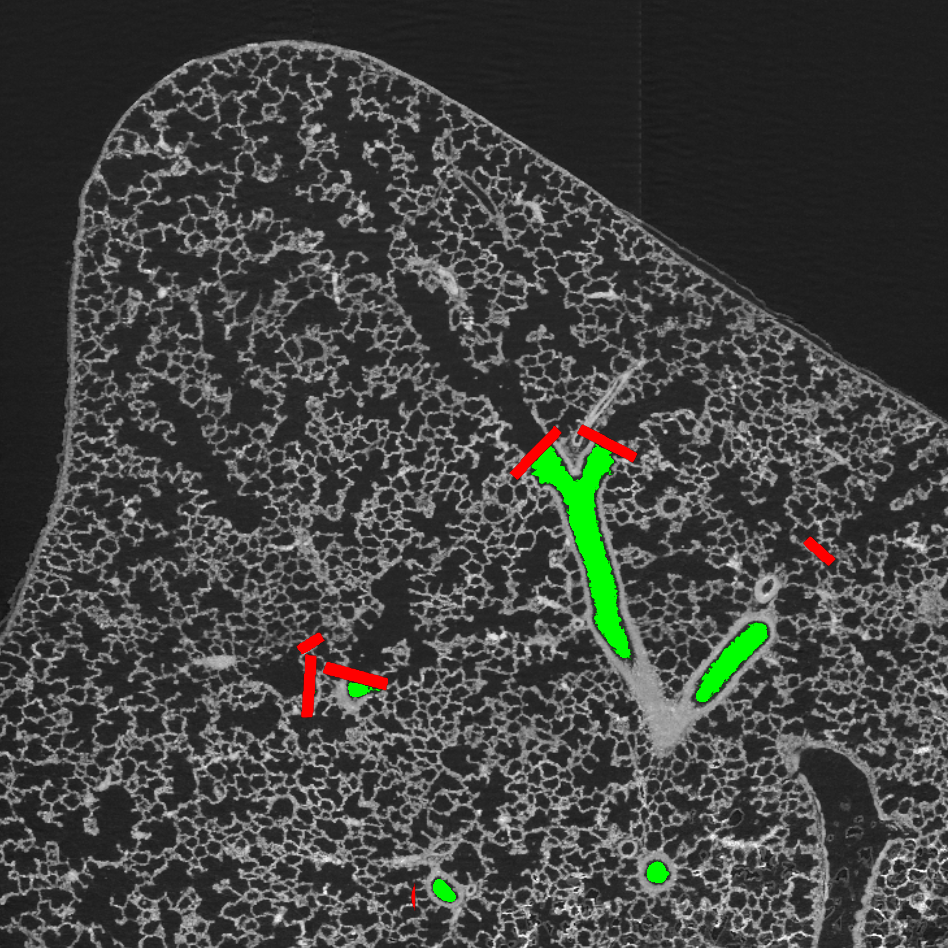
\includegraphics[width=\imagewidth]{img/ManholeCoverExplanation/60B_sagittal_slice_415}}; %_scalebar
		% 440px = 2mm > 100px = 455um > 110px = 500um, 22px = 100um
		%\draw[|-|,blue,thick] (868,237) -- (868,677) node [sloped,midway,above,fill=white,semitransparent,text opacity=1] {\SI{2}{\milli\meter} (2000px) TEMPORARY!};
		\draw[|-|,white,thick] (\x,\y) -- (\x+110,\y) node [midway,above] {\SI{500}{\micro\meter}};
		\draw[yellow,dashed,ultra thick] (508,436) circle (20);
		\fill[yellow,nearly transparent] (508,436) circle (20);
		\draw[yellow,dashed,ultra thick] (617,407) circle (20);
		\fill[yellow,nearly transparent] (617,407) circle (20);
		\draw[yellow,dashed,ultra thick] (642,434) circle (20);
		\fill[yellow,nearly transparent] (642,434) circle (20);
		\draw[yellow,dashed,ultra thick] (385,663) circle (20);
		\fill[yellow,nearly transparent] (385,663) circle (20);	
		\draw[yellow,dashed,ultra thick] (347,653) circle (15);
		\fill[yellow,nearly transparent] (347,653) circle (15);
		\draw[yellow,dashed,ultra thick] (245,667) circle (20);
		\fill[yellow,nearly transparent] (245,667) circle (20);	
	\end{tikzpicture}%
	\caption{One sagittal slice of the tomographic dataset of the animal B showing extracted conducting airways in green and several manhole covers in red. The dashed yellow circles highlight some examples of alveolar outpouchings of the airway wall which mark the change from conducting to gas-exchanging regions. Additionally, changes in the epithelial layer of the airway wall, especially changes in thickness and structure also mark this change. Visually assessing these changes made it possible to semi-automatically place manhole covers in the three-dimensional tomographic dataset to isolate single acini from our dataset. Four manhole covers are shown cut right through the middle, two manhole covers are cut fractionally and thus appear much smaller on this slice.}
	\label{fig:ManholeCoverExplanation}
\end{figure}

Once all acinar entrance points were defined, we extracted the volume of each isolated acinus (shown as yellow volumes in \autoref{subfig:extracted acini}) in an automated third step. The manhole covers placed in the steps mentioned before are defined through their diameter and \href{https://secure.wikimedia.org/wikipedia/en/w/index.php?title=Surface_normal&oldid=411684319}{surface normal} in the three-dimensional dataset. We extracted the volume of the single acini using an additional region growing module. The seed point for this additional module was defined in such a way that we simply flipped the direction of the surface normal defining the manhole cover and placed the seed point for the acinar region growing along this vector, slightly behind the manhole cover inside the acinar airspace. The only manual work needed for the final extraction of the volume of each acinus was the iterative selection of the appropriate segmentation threshold and subsequent tabulation of the automatically calculated acinar volume.

\renewcommand{\imsize}{0.33\linewidth}%
\pgfmathsetlength{\imagewidth}{\imsize}%
\pgfmathsetlength{\imagescale}{\imagewidth/800}%
\def\x{10}% scalebar-x at golden ratio of x=800px
\def\y{750}% scalebar-y at 90% of height of y=800px
\begin{figure}
	\centering
	\subfloat[Sample]{%
		\begin{tikzpicture}[x=\imagescale,y=-\imagescale]
			\node[anchor=north west, inner sep=0pt, outer sep=0pt] at (0,0) {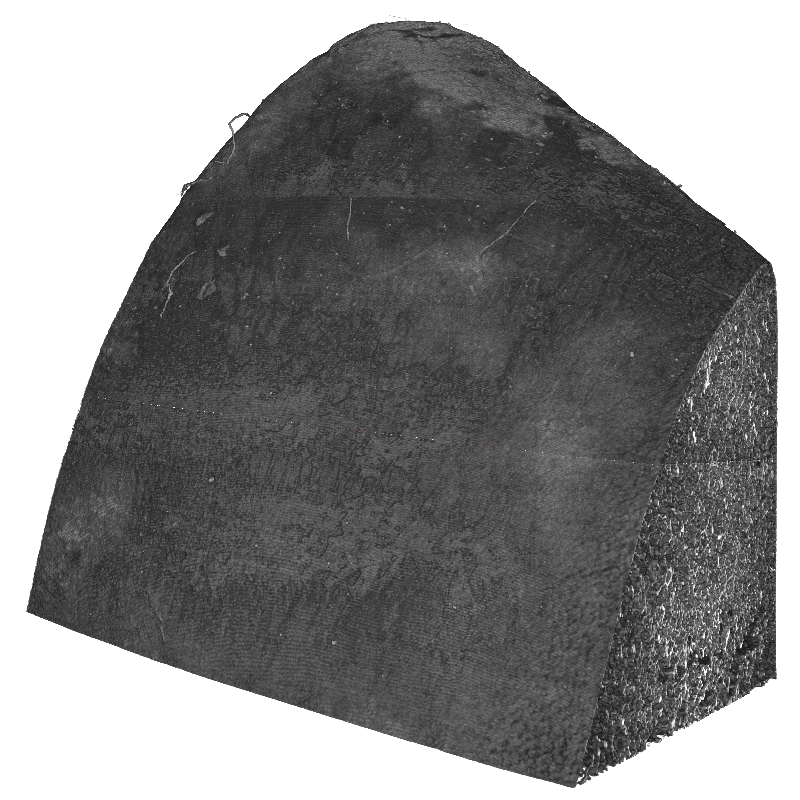
\includegraphics[width=\imagewidth]{img/ManholeCover/R108C60B_2010c_Sample}};
			% 570px = 4.363mm > 100px = 765um > 65px = 500um, 13px = 100um
			%\draw[|-|,blue,thick] (30,608) -- (571,788) node [sloped,midway,above,fill=white,semitransparent,text opacity=1] {\SI{4.363}{\milli\meter} (2948px) TEMPORARY!};
			\draw[|-|,thick] (\x,\y) -- (\x+65,\y) node [right] {\SI{500}{\micro\meter}};
		\end{tikzpicture}%
		\label{subfig:sample}%
		}%
	\subfloat[Extracted conducting airways with manhole covers shown overlaid over Sample.]{%
		\begin{tikzpicture}[x=\imagescale,y=-\imagescale]
			\node[anchor=north west, inner sep=0pt, outer sep=0pt] at (0,0) {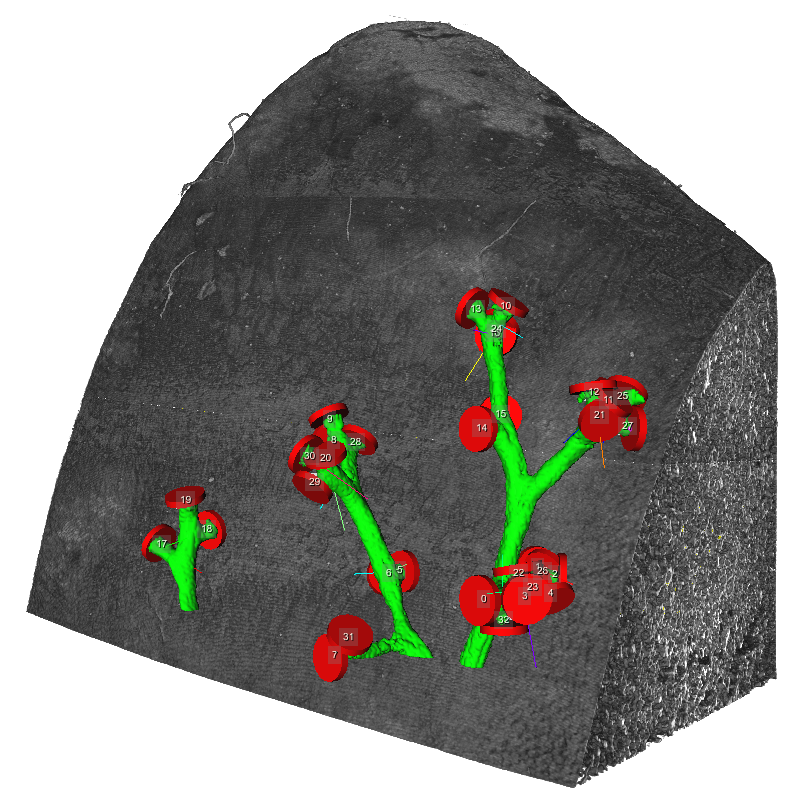
\includegraphics[width=\imagewidth]{img/ManholeCover/R108C60B_2010c_Sample_Airway}};
			\draw[|-|,thick] (\x,\y) -- (\x+65,\y) node [right] {\SI{500}{\micro\meter}};
		\end{tikzpicture}%
		\label{subfig:airway segment}%
		}%
	\subfloat[Extracted acini.]{%
		\begin{tikzpicture}[x=\imagescale,y=-\imagescale]
			\node[anchor=north west, inner sep=0pt, outer sep=0pt] at (0,0) {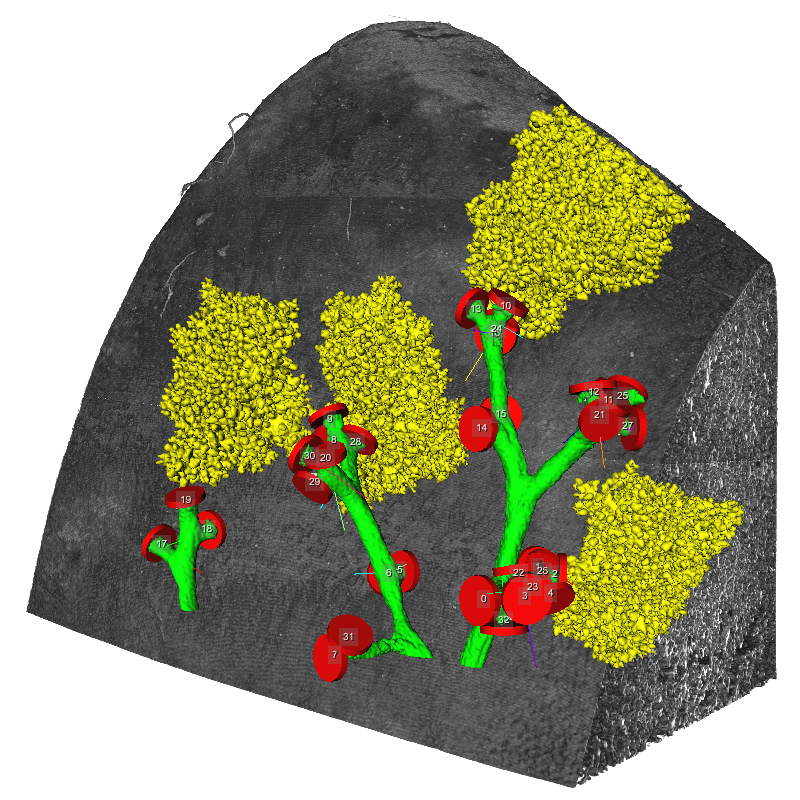
\includegraphics[width=\imagewidth]{img/ManholeCover/R108C60B_2010c_Sample_Acini}};
			\draw[|-|,thick] (\x,\y) -- (\x+65,\y) node [right] {\SI{500}{\micro\meter}};§
		\end{tikzpicture}%
		\label{subfig:extracted acini}%
		}
	\caption{Visualization of the work flow for the extraction of the acinar volumes on a rat lung sample extracted at day 60: %
		\protect\subref{subfig:sample}: three-dimensional visualization of a sample. To increase the field of view nine-fold compared to a classic scan at TOMCAT we stacked three wide field scans on top of each other. The borders between the three stacked scans are faintly visible as darker lines, but are only visible in this three-dimensional visualization and did not influence the three-dimensional reconstruction. %
		\protect\subref{subfig:airway segment} Extracted airway segment (green) superimposed on the sample. Using a threshold based region growing algorithm, we extracted conducting airways inside the sample. The red discs shown are the so-called manhole covers, which were semi-automatically placed and used as segmentation stoppers for the region growing. %
		\protect\subref{subfig:extracted acini} Extracted acini (yellow). Several extracted acini are shown superimposed over the sample in three-dimensional. For each such acinus we recorded the volume.%
		}
	\label{fig:workflow}
\end{figure}

The volume of the single acini was calculated by multiplying the number of segmented voxels with the voxel volume. The single acini were exported to \href{https://secure.wikimedia.org/wikipedia/en/w/index.php?title=Digital_Imaging_and_Communications_in_Medicine&oldid=415023605}{DICOM} files for further processing as described below. The files contained the volume segmented as described above overlaid over the corresponding region of interest of the original tomographic dataset in the background. The filename of these files was composed of the sequential number of the acinus and its volume. Since we also recorded the exact location of the seed points and threshold used to segment the acinus, the extraction of the single acini is exactly reproducible.

\subsection{Stereological Analysis}
The volume of the single acini was automatically calculated from the amount of segmented voxels multiplied by their size. To check these volumes against a gold standard method, we stereologically estimated the volume of single exemplary acini. To guarantee accurate and unbiased results, we standardized each step of tissue fixation, processing sampling and analysis and performed the stereological assessment according to official guidelines, as specified by \citet{Hsia2010}.

For this analysis, we prepared datasets in which we combined each segmented acinus with the corresponding region of interest from the original tomographic dataset, as seen in the background of \autoref{fig:STEPanizer} and exported these regions of interest as DICOM files. With a MATLAB script we padded the volumes to a square format, performed a systematic random sampling of slices and exported the selected as JPG sequences for the stereological analysis.

Using a web based tool developed at our institute, the so-called STEPanizer~\cite[available free of charge at \url{http://stepanizer.com}]{Tschanz2011} we analyzed the volume and surface of the extracted acini. Intersections of the acinar surface with geometric line probes were counted to assess the acinar surface, while simple point counting was used to assess the volume of the extracted acini and the ratio of in- and out-of-sample volume.

\autoref{fig:STEPanizer} shows one such exported slice while being analyzed using the STEPanizer. Counting points (green three-quarter circles) and intersections (red \href{https://encrypted.google.com/search?q=i-beam&tbm=isch}{I-beam}-shaped lines) are overlaid to count both the points inside the acinar volume and intersections with the acinar surface. The measurements are exported to \href{https://secure.wikimedia.org/wikipedia/en/w/index.php?title=Comma-separated_values&oldid=441921632}{csv}-delimited tables for further analysis. This process made it possible to relate the automatically calculated volumes from MeVisLab to an accepted and proven stereological method.

\renewcommand{\imsize}{\linewidth}%
\pgfmathsetlength{\imagewidth}{\imsize}%
\pgfmathsetlength{\imagescale}{\imagewidth/1280}%
\begin{figure}
	\centering
	\begin{tikzpicture}[x=\imagescale,y=-\imagescale]
		\node[anchor=north west, inner sep=0pt, outer sep=0pt] at (0,0) {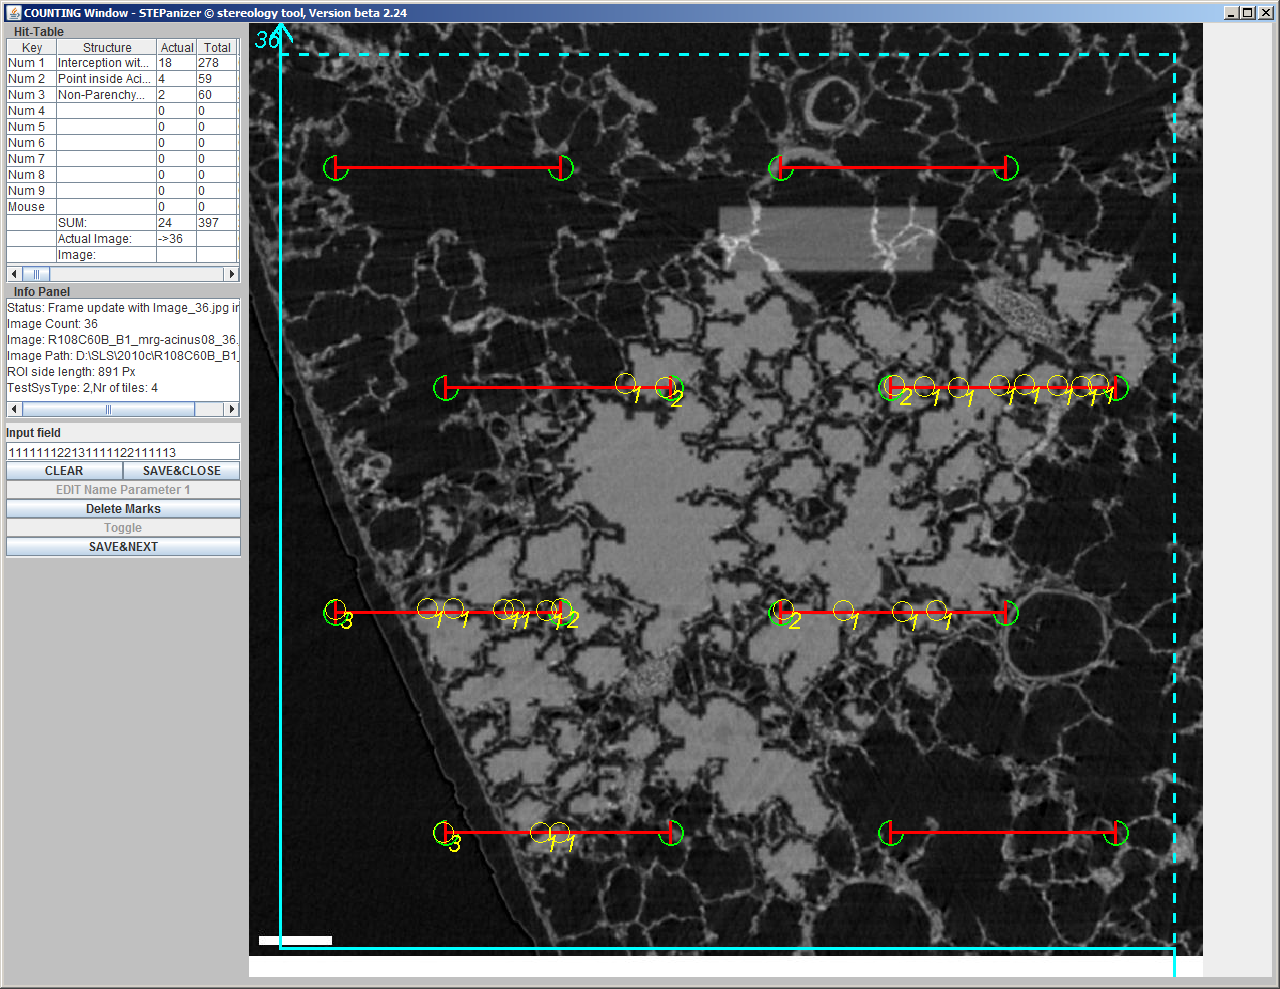
\includegraphics[width=\imagewidth]{img/STEPanizer_2010_R108C60B_acinus08_Slice36}};
		% 914px = 0.1mm > 100px = 11um > 4568px = 500um, 914px = 100um
		\draw[dashed,green,thick] (719,207) -- (937,207) -- (932,270) -- (723,270) -- cycle ;
	\end{tikzpicture}%
	\caption{STEPanizer counting window. The segmented acinus is visible in light gray, the manhole cover which was used to separate this acinus is visible in the upper right region (marked with a dashed green line which is originally not visible in the STEPanizer). Both structures have been merged with the original tomographic data using the described MeVisLab work flow and exported to single jpg files. Line and point probes (red lines and green circles) are overlaid over the image for counting. To correctly count all structures in the image, the original non-square datasets have been padded to a square, resulting in the small white rectangle at the lower border of the image. Scalebar: \SI{100}{\micro\meter}.}
	\label{fig:STEPanizer}
\end{figure}

Using a \href{http://python.org/}{Python} script\todo{Can we attach it to provide the data for \href{http://reproducibleresearch.net/index.php/Main_Page}{reproducible research}?}, we extracted and calculated the volume assessed with MeVisLab and the STEPanizer for 43 acini from their respective files, the results are presented in \autoref{sec:results} below.

\section{Results}
\label{sec:results}
\subsection{Acinar Volume}
% Mean acinar volume for single samples
% R108C60A: not measured
% R108C60B_B1_mrg: 0.001 cm^3
% R108C60C: not measured
% R108C60Dt-mrg: 0.002 cm^3
% R108C60Et-mrg: 0.002 cm^3
% Mean acinar volume for all samples: 0.002 cm^3
% Standard deviation of the mean acinar volume for all samples: 0.000624982186542
We extracted and stereologically analyzed several acini from tomographic datasets. The data we show here consists of \numberofacini\xspace analyzed acini, their mean volume is \SI{\volume}{\centi\metre\cubed}, with a standard deviation of \SI{\std}{\centi\metre\cubed}.

\subsection{Number of Acini}
% Number of acini (= absolute airspace volume from stefan / mean acinar volume)
% R108C60A was not measured
% R108C60B_B1_mrg contains 8279 acini
% R108C60C was not measured
% R108C60Dt-mrg contains 4486 acini
% R108C60Et-mrg contains 2928 acini

% Rodriguez1987 (page 146) states a total of 4023 acini for the whole rat lungs.
% We have a *mean* of 5231 acini calculated for the whole lung.
For the three different animals we estimated an absolute number of acini for the whole lung by dividing the absolute parenchymal volume of the lung by the mean acinar volume and obtained 8279, 4486 and 2928 acini for the animals R108C60B, R108C60D and R108C60E, respectively. The mean number of acini for the whole lung is thus calculated to be 5231 acini. 

\subsection{Acinar surface and total diffusion surface}
%Mean acinar surface for single samples
%R108C60A: not measured
%R108C60B_B1_mrg: 0.466 cm^2
%R108C60C: not measured
%R108C60Dt-mrg: 0.702 cm^2
%R108C60Et-mrg: 1.102 cm^2
%Mean acinar surface for all samples: 0.756 cm^2

%Diffusion surface (=number of acini * mean acinar surface)
%R108C60A was not measured
%R108C60B_B1_mrg contains 3856.407 cm^2 of diffusion surface
%R108C60C was not measured
%R108C60Dt-mrg contains 3148.369 cm^2 of diffusion surface
%R108C60Et-mrg contains 3225.448 cm^2 of diffusion surface
%
%Stefan measured the absolute airspace surface with EM and got
%R108C60A: 7417.908 cm^2
%R108C60B_B1_mrg: 7667.099 cm^2
%R108C60C: 10396.943 cm^2
%R108C60Dt-mrg: 7448.81 cm^2
%R108C60Et-mrg: 7173.484 cm^2
%
%Stefans mean absolute airspace surface is 8020.849 cm^2.
%Our mean airspace surface is 3410.074 cm^2.Standard deviation of the mean acinar surface for all samples: 0.262469473252
To automatically extract the surface of the single acini a triangulation of the surface would be needed, \ie the extent of the voxels has to be mapped to adjoining triangles in the three-dimensional space. Since the triangulation of the surface inherently poses a classic \emph{Coast of Wales}-problem~\cite{Mandelbrot1967a} and is heavily depending on the resolution of the used dataset, we did not automatically calculate the surface (\eg using MeVisLab), but stereologically estimated the the surface of the acini by counting interception of test lines with the acinar septa \cite{Hsia2010}.

For the three different animals we calculated a mean acinar surface of \SI{0.756}{\centi\metre\squared} (R108C60BB: \SI{0.466}{\centi\metre\squared}, R108C60D: \SI{0.702}{\centi\metre\squared} and R108C60E: \SI{1.102}{\centi\metre\squared}). With the number of acini calculated above, this translates to a mean diffusion surface of \SI{3410}{\centi\metre\squared} (R108C60B: \SI{3856}{\centi\metre\squared}, R108C60D: \SI{3148}{\centi\metre\squared} and R108C60E: \SI{3225}{\centi\metre\squared}).

\subsection{Comparison of Volumes from MeVisLab with STEPanizer}
% MeVisLab volume compared to STEPanizer volume (STEPanizer/MeVisLab)
% In mean, (STEPanizer-/MeVisLab-volume) is 3.133
For \numberofacini\xspace acini of three different animals we automatically assessed the volume by adding the segmented voxels inside the acini and multiplying them with the voxel volume and estimated the volume with the manual Cavaglieri method \cite{Hsia2010} using the STEPanizer. The results are shown in \autoref{fig:VolumeMeVisVsSTEPanizer} and explained later on in the Discussion section. Normalizing the volumes to the largest acinus shows that while both methods result in different volumes, they scale in the same range, see \autoref{fig:VolumeMeVisVsSTEPanizerNormalized}.

\renewcommand{\imsize}{\linewidth}
\begin{figure}[htb]
\centering
 	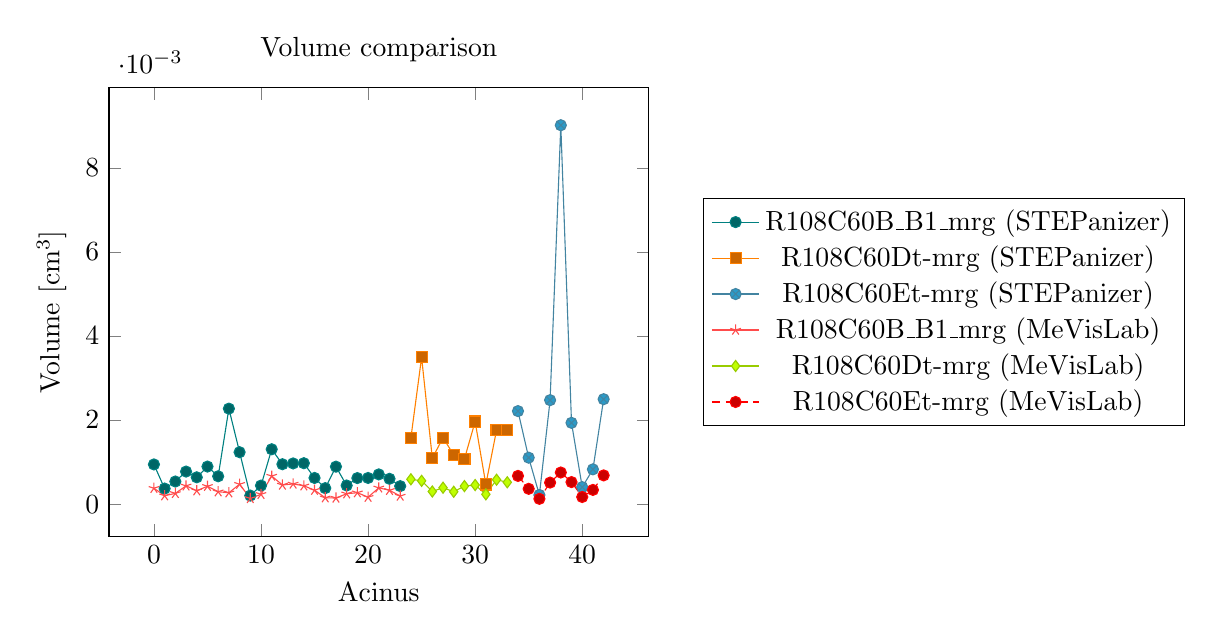
\begin{tikzpicture}
	 	\begin{axis}[
	 		cycle list name = exotic,
	 		title={Volume comparison},
			xlabel={Acinus},
			ylabel={Volume [\si{\centi\metre\cubed}]},% \si{\cubic\centi\meter},
			legend entries={R108C60B\_B1\_mrg (STEPanizer),R108C60Dt-mrg (STEPanizer),R108C60Et-mrg (STEPanizer),R108C60B\_B1\_mrg (MeVisLab),R108C60Dt-mrg (MeVisLab),R108C60Et-mrg (MeVisLab)},
			legend style={
				at={(1.1,0.5)},
				anchor=west
				%legend columns=3,
				%font=\tiny,
				%rounded corners = 3,
				%at={(0.5,-0.25)},
				%anchor=north
				},
			%width=\imsize
			]
			\addplot % [draw,fill=red,red=square*]
				coordinates {
					(0,0.000943978089591402) (1,0.000369290006731552) (2,0.000537284135255814) (3,0.000774104716030111) (4,0.00063721303615683) (5,0.000892998673456294) (6,0.			000662060213607909) (7,0.00227213474409444) (8,0.00123480580445082) (9,0.000202540993042524) (10,0.000440456598544131) (11,0.00130506260473565) (12,0.		000948905265220132) (13,0.000967796840998029) (14,0.000973053509272693) (15,0.000622005326109383) (16,0.0003792715403106) (17,0.00089103877005466) (18,0.000442312679892422) (19,0.000618971153786899) (20,0.000622005326109383) (21,0.000706693979639465) (22,0.000602002519342455) (23,0.000427844990797474) 
					};
			\addplot %[draw,fill=green,only marks,mark=square*]
				coordinates {
					(24,0.0015775832244119) (25,0.00349411900606628) (26,0.00109353123999124) (27,0.00157806449893873) (28,0.00117142214981822) (29,0.0010757778774242) (30,0.0019641417554389) (31,0.000467836408179399) (32,0.00176092960260168) (33,0.00176717628474684) 
					};		
			\addplot %[draw,fill=blue,only marks,mark=square*]
				coordinates {
					(34,0.00221322926506789) (35,0.00110468828837077) (36,0.000217300159958048) (37,0.00247446056987033) (38,0.00901848490761219) (39,0.00193425723370187) (40,0.000404056440325775) (41,0.000827363638248959) (42,0.00249739786677173) 
					};		
			\addplot %[draw,fill=red,only marks,mark=*]
				coordinates {
					(0,0.00037731293) (1,0.00019965522) (2,0.00025447792) (3,0.00043383464) (4,0.00031837037) (5,0.00042459121) (6,0.000294278) (7,0.00026970762) (8,0.00047316542) (9,0.00013395399) (10,0.0002331105) (11,0.00066745716) (12,0.00045502964) (13,0.00047915584) (14,0.00043513966) (15,0.00033121431) (16,0.00015090302) (17,0.00014413643) (18,0.00024587891) (19,0.00027121842) (20,0.00016399051) (21,0.00038648456) (22,0.00032862523) (23,0.00019227928) 
					};
			\addplot %[draw,fill=green,only marks,mark=*]
				coordinates {
					(24,0.0005900293) (25,0.00055371433) (26,0.00029986489) (27,0.00039014131) (28,0.00029307008) (29,0.00042841768) (30,0.0004532719) (31,0.00023229824) (32,0.00058026904) (33,0.00051905155) 
					};
			\addplot %[draw,fill=blue,only marks,mark=*]
				coordinates {
					(34,0.0006709888) (35,0.00036325091) (36,0.00012486846) (37,0.00051163185) (38,0.00075202513) (39,0.00052375108) (40,0.00016866906) (41,0.00033741882) (42,0.00068318522) 
					};
			\end{axis}
	\end{tikzpicture}
	\caption{Volumes of different acini estimated with different Methods.}
	\label{fig:VolumeMeVisVsSTEPanizer}%
\end{figure}

As expected, both methods show different results; the volumes of single acini assessed with the stereological method show a \difference\(\times\) larger value than when assessed with the automatic method using voxel counting. Since the automatic calculation of the acinar volume with MeVisLab simply adds up all segmented voxels, an imprecise segmentation leads to an underestimation of the acinar volume. \autoref{fig:MeVisSegmentation} shows exemplary slices for acini with large differences in volume between the two methods. Due to inevitable segmentation inaccuracies (dark spots inside the segmented acinus in \autoref{subfig:60d_acinus32} we underestimated the volumes with the automatic method compared to the manual, stereological method, where we easily can discard such inaccuracies due to manual work.

In some extracted acini we have seen differences in gray values in the z-direction of the stack. Since the region growing segmentation method uses the same threshold throughout the region of interest, sometimes single slices were heavily under-estimated in terms of included voxels, one such example is shown in \autoref{subfig:60e_acinus38}. Since these automatically extracted regions were merely used as a optic guidance for the manual, stereological method it is obvious that the manual method shows slightly larger and more accurately estimated volumes than the automatic method.

\section{Discussion}
Applying our novel method dubbed manhole cover segmentation to tomographic datasets of three animals we extracted more than 40 acini for three different animals from nondestructively acquired tomographic datasets. The simple extraction of single acini permits us to analyze parameters like volume and surface of single acini and total number of acini and diffusion surface in the mammalian lung.

Using our semiautomatic method we are able to isolate and analyze individual acini in both a two- and three-dimensional way using widely accepted methods like voxel counting and Stereology. We have shown that we can automatically calculate the volume of single acini in mammalian lungs from three-dimensional tomographic data and match the accuracy of a manual method while performing the analysis orders of magnitude faster. Only with this novel combination of methods it is possible to accurately assess the volume of single acini in three-dimensional tomographic data.

Our proposed method opens up the possibility to fully analyze biologically interesting parameters of the acini in the lung; the volume of the acini can be extracted automatically, parameters like surface as well as number of contained alveoli and septal length per acinus can be extracted with simple stereological counting, requiring manual labor.

With the proposed method we can additionally analyze structural changes in the acinus over the postnatal development. Structural changes during development, like disease or differences between wild-type and knock-out animals can be analyzed. All the parameters mentioned above and the structural changes can be obtained for single isolated acini, something which is not easily possible using stereological methods on classic tissue sections.

\subsection{Acinar Volume}
\citet[Table 1]{Rodriguez1987} found that the right upper lobe of one rat contains 613 acini with a mean volume of \SI{1.98}{\milli\meter\cubed} (\SIrange{0.5}{5}{\milli\meter\cubed}). Our calculations resulted in a volume of \SI{\volume}{\cubic\centi\meter} with a standard deviation of \SI{\std}{\cubic\centi\meter}, which corresponds to \SI{1.554}{\cubic\milli\meter}. The stereologically estimated mean acinar volume is thus in the range of previously published data.\todo{Is there more data we can/should relate to?}

\subsection{Number of acini}
We found a mean number of approximately 5000 per rat lung for our three animal. \citet[page 146]{Rodriguez1987} found a total of 4023 acini in the whole lungs for one single rat\todo{Other data?}. We did not directly assess the number of acini \todo{Eveline did!!!}, but only estimated the total number of acini by dividing the absolute airspace volume \todo{Citation DatenblattStefan.xls} by the mean acinar volume. Even though our values are a crude approximation of the acinus number, our results are comparable to published results up to now, showing the feasibility of our method.

\subsection{Acinar surface and total diffusion surface}\todo{is there data we can discuss here?}
Missing other published data, we can only relate the assessed alveolar surface to other mean values found in literature, namely the absolute airspace surface in the rat lung, which has been assessed by Tschanz et al\todo{Did Stefan publish this data somewhere? Cite it!}. Tschanz et al. assessed the absolute airspace surface by stereological estimation using electron microscopy images and found a mean absolute airspace surface of \SI{8021}{\centi\metre\squared} for the same five rat lungs we assessed\todo{Are these really the same animals?}. By multiplying the number of acini by the mean acinar surface we found the mean absolute airspace surface to be \SI{3410}{\centi\metre\squared}, roughly 2.4\(\times\) smaller than Tschanz et al.\todo{Can we explain the difference with the difference of the two methods?}

\subsection[Comparison of MeVisLab with STEPanizer]{Comparison of automatic Stereology with MeVisLab and manual Stereology with the STEPanizer}
Manually assessing the volume of the single acini using the STEPanizer took several working days for the few acini shown in \autoref{fig:VolumeMeVisVsSTEPanizer}. As soon as the manhole covers are defined in the sample, the automatic volume calculation with MeVisLab can be performed in an automatic way in less than a minute per acinus. Even though we underestimate the volume of the single acini with the automatic method, we still would not rule out completely the manual method, especially if looking at very large numbers of acini\todo{Do we never mention the 1000 acini I totally extracted?}.

The difference between the automatic and manual volume estimation (MeVisLab or STEPanizer, respectively) is explained by the differences in the method (single voxel counting vs.\ manual, global stereological assessment). The under-estimation of the volume with the automatic method is inherently based in the method itself, \ie since we simply add up segmented voxels. Thus, fluctuations in the grey value of the raw data can lead to an imprecise segmentation with missing voxels which are then not counted for the acinar volume. Nonetheless, since the automated volume extraction is extremely faster than the manual, stereological assessment of the acinar volumes, we feel that the proposed method is of great value nonetheless. Additionally, since the segmentation of single acini is anyways the prerequisite for the stereological assessment of these single acini and represents the main amount of time spent evaluating the data, the automatic extraction of the volume can be automatically performed in a very short time.

We thus propose that---if absolute values are needed for a larger study---the automatic extraction of the volume is calibrated against the gold standard, the manual, stereological assessment of the volume according to \citet{Hsia2010}. Since for our planned follow-up study we will not look at the absolute volume, but only at the volume fractions or increase of volume, the difference in absolute volume between the two methods can be neglected for our purposes.

\renewcommand{\imsize}{0.56\linewidth}%
\begin{figure}
	\centering
	\hfill%
	\subfloat[60D, Acinus 32, Slice 45, Vol.\ \SI{159}{\percent}]{%
		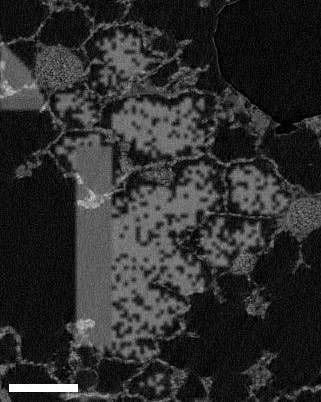
\includegraphics[height=\imsize]{img/Acini/2009f/mrg/R108C60Dt-mrg/acinus32/voxelsize1.48-every6slice/R108C60Dt-mrg-acinus32_45.png}% jpg is unedited!
		\label{subfig:60d_acinus32}%
	}%
	\hfill%
	\subfloat[60E, Acinus 38, Slice 29, Vol.\ \SI{188}{\percent}]{%
		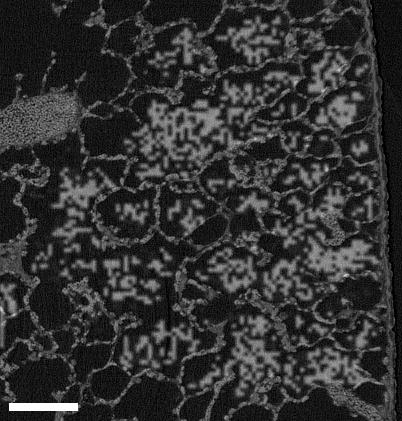
\includegraphics[height=\imsize]{img/Acini/2009f/mrg/R108C60Et-mrg/acinus38/voxelsize1.48-every6slice/R108C60Et-mrg-acinus38_29.png}% jpg is unedited!
		\label{subfig:60e_acinus38}%		
	}%
	\hfill%
	\caption{Illustrative slices of two acini that show large differences in volume between MeVisLab and STEPanizer. The inaccurate segmentation is the reason we obtained larger volumes with the STEPanizer than with MeVisLab. Panel \protect\subref{subfig:60d_acinus32} shows minor segmentation errors through noise in the paraffin (dark spots inside grey region). Panel \protect\subref{subfig:60e_acinus38} shows large segmentation errors. Such large errors arise through brightness changes in the dataset which render the global threshold unusable for certain slices. Scale bar: \SI{100}{\micro\meter}.}
	\label{fig:MeVisSegmentation}
\end{figure}

\subsection{Conclusions}
The hereby presented manhole cover method is well suited to semi-automatically isolate single acini from three-dimensional datasets for further stereological analysis. To our knowledge, the presented work flow is the only one published to permit a semiautomatic extraction of single acini. After the extraction of single acini, a fully automated calculation of the volume of individual acini is possible, thus for the first time enabling the study of large amounts of individual acini in relatively short time.\todo{Shall we write something about the 1000 extracted acini for days \numrange{4}{60}?}. This opens up the possibility to efficiently estimate biological parameters like volume and surface of single acini, number of acini and diffusion surface in the mammalian lung using accepted stereological methods.

We validated our automatic method with a proven and accepted method, the so-called Stereology. We have shown that---even though there are differences between the two methods---the achieved results are comparable. Since our proposed method for assessing the volumes of isolated individual acini is by magnitudes faster than manual stereological counting, we believe the presented method is the easiest and fastest way to assess the volume of single acini in the mammalian lungs.

\clearpage
\section{Acknowledgments}
We thank Federica Marone, Christoph Hintermüller and Bernd Pinzer for the great support at the TOMCAT Beamline. Milo Hindennach from Fraunhofer MEVIS provided the \href{http://www.mevis-research.de/cgi-bin/discus/board-auth.cgi?lm=1282233250&file=/839/11760.html}{Manhole cover module in MeVisLab}. We thank Mohammed Ouanella and Eveline Yao for expert technical assistance and embedding of the samples.

This work has been funded by the grants 3100A0-109874 and 310030-125397 of the Swiss National Science Foundation.

\clearpage
\singlespacing
\bibliographystyle{plainnat}
\bibliography{../library}

\end{document}